% Figure from MATH 493 notes, section 47 (review session 10/21). Compile with the notes preamble.
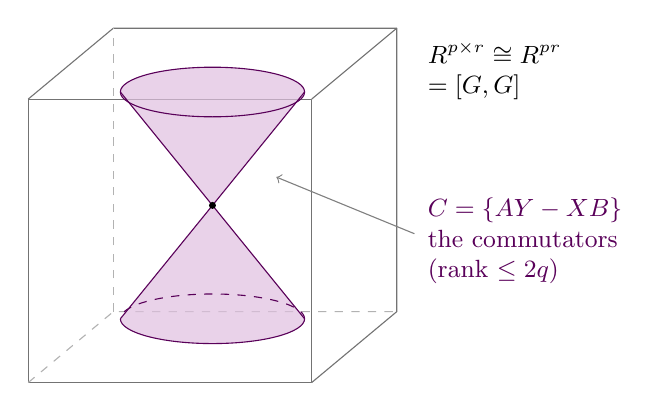
\begin{tikzpicture}[scale=0.9, line join=round]
  \draw[black!55] (0,0) rectangle (4,4);
  \draw[black!55] (4,0) -- (5.2,1) -- (5.2,5) -- (4,4);
  \draw[black!55] (0,4) -- (1.2,5) -- (5.2,5);
  \draw[black!30, dashed] (0,0) -- (1.2,1) -- (5.2,1);
  \draw[black!30, dashed] (1.2,1) -- (1.2,5);
  \fill[violet!25, opacity=0.7] (1.3,4.1) -- (2.6,2.5) -- (3.9,4.1) arc (0:180:1.3 and 0.35) -- cycle;
  \fill[violet!25, opacity=0.7] (1.3,0.9) -- (2.6,2.5) -- (3.9,0.9) arc (0:-180:1.3 and 0.35) -- cycle;
  \draw[violet!70!black] (2.6,4.1) ellipse (1.3 and 0.35);
  \draw[violet!70!black] (1.3,4.1) -- (3.9,0.9);
  \draw[violet!70!black] (3.9,4.1) -- (1.3,0.9);
  \draw[violet!70!black] (1.3,0.9) arc (180:360:1.3 and 0.35);
  \draw[violet!70!black, dashed] (3.9,0.9) arc (0:180:1.3 and 0.35);
  \fill (2.6,2.5) circle (1.4pt);
  \node[font=\small, align=left, anchor=west] at (5.5,4.4) {$\mathbb{R}^{p \times r} \cong \mathbb{R}^{pr}$\\ $= [G,G]$};
  \node[font=\small, text=violet!70!black, align=left, anchor=west] at (5.5,2.0) {$C = \{AY - XB\}$\\ the commutators\\ (rank $\leq 2q$)};
  \draw[->, black!50] (5.45,2.1) -- (3.5,2.9);
\end{tikzpicture}
